%!TEX root = ../template.tex
%%%%%%%%%%%%%%%%%%%%%%%%%%%%%%%%%%%%%%%%%%%%%%%%%%%%%%%%%%%%%%%%%%%%
%% chapter4.tex
%% NOVA thesis document file
%%%%%%%%%%%%%%%%%%%%%%%%%%%%%%%%%%%%%%%%%%%%%%%%%%%%%%%%%%%%%%%%%%%%

\typeout{NT FILE chapter4.tex}%

\chapter{Solution}
\label{cha:solution}

\prependtographicspath{{Chapters/Figures/Covers/}}

\glsresetall
 
\section{Threat Modeling Protocol for Horizontal Organizations}
\label{sec:protocol}

Horizontal cooperatives face unique security challenges. Without a central
authority, they are vulnerable to attacks that exploit their open, democratic
nature. For example, an attacker might create fake member identities to sway
decisions or abuse the consensus process to cause chaos. At the
same time, horizontality can be a security strength: distributing decisions
means there is no single point of failure. This protocol treats horizontality
as an asset, making security a collective endeavor rather than a top-down
mandate.

\subsection{Key Design Principles}
\label{subsec:key_principles}

\begin{itemize}
    \item \textbf{Transparency}: Security activities like decisions,
configurations and incidents should be visible to members. Open logs and
auditable records ensure nothing happens behind closed doors, building trust
and accountability among the group.
    \item \textbf{Decentralization}: No single person should have unchecked
power over systems or data. Access and control are distributed. This prevents a
single admin from being a weak link and avoids creating a digital vanguard
where a tech-savvy few hold all the keys.
    \item \textbf{Democratic Participation}: All members can participate in
identifying and addressing threats. Security decisions are made through
inclusive discussions or votes, so measures are collective. This keeps
the process aligned with the coop's democratic governance.
    \item \textbf{Traceability}: Every important action like granting access or making
a change leaves an immutable trail. For example, changes can be logged on
tamper-proof ledgers and digitally signed by those who approved them. This way,
if something goes wrong, the coop can trace what happened and who was involved,
without relying on memory or hearsay.
    \item \textbf{Resilience}: The protocol aims to strengthen the coop's
ability to withstand and recover from threats. By eliminating single failure
points and planning for crises with backup plans and rapid response
mechanisms, the organization stays resilient even under attack.
\end{itemize}

These principles ensure that improving security will not undermine the
organization nature of the group. Instead, security measures will reinforce
collaboration, shared responsibility, and trust. In practice, this means
building security into everyday cooperative workflows and governance. What
follows is a step-by-step threat modeling process designed with these values in
mind. It's written in accessible language so that any member can take part.
Each step includes guidance and checklists for participatory activities,
and the protocol can be scaled or adapted for organizations of different
sizes and structures.

Note: While this protocol is inspired by established frameworks like PASTA,
it does not use the formal seven-stage PASTA terminology. Instead, it
presents an equivalent logic in a more accessible format focusing on
horizontal scenarios.

\subsection{Target Audience}
\label{subsec:target_audience}

The protocol is designed for members of horizontal organizations without
specialized cybersecurity expertise. Unlike traditional expert-oriented models,
our protocol emphasizes simplicity and accessibility. It supports stakeholders
involved in decision-making, operational activities, conflict resolution, and
coordination tasks, as well as informal community groups, by providing clear
guidance and intuitive methods for effectively dealing with security threats.

\subsection{Ethics and Protection of Organizations}
\label{subsec:ethics_protection}

When constructing and applying the threat modeling protocol in non-hierarchical
organizations, it is imperative to consider ethical principles as structuring
elements that transcend the merely technical aspect of cybersecurity. Ethical
concerns are based on the explicit commitment to protecting not only
technological integrity, but also the individuals and groups involved in
organizational processes.

A crucial aspect in this context is the responsibility regarding the
confidentiality of sensitive information and the protection of the privacy of
organizational members. The inadvertent exposure of security flaws can cause
significant damage, not only operational, but also personal and social.
Therefore, the protocol must incorporate strict guidelines on the ethical
treatment of identified vulnerabilities, ensuring that such information is
managed in a restricted manner and shared only with authorized individuals or
groups.

Additionally, it is vital to establish clear internal communication mechanisms
to ensure that any identified vulnerabilities are immediately reported,
mitigated and documented without unnecessary public exposure.

\section{Threat Modeling Process Overview}
\label{sec:threat_modeling_process_overview}

The threat modeling process is broken into eight collaborative steps. In a small
cooperative, most steps can be taken in all-hands meetings or workshops with
everyone. In larger groups, you might delegate initial work to
working groups, but every member should have a chance to review and contribute
at each stage. The process is iterative and modular, so you can adjust the depth
or format of each step based on your organization's size and needs. For each
step below we describe the process and its activities
along with tips to adapt to different situations.

\subsection{Step 1: Establish Context and Goals}
\label{subsec:Step1}

What Are We Protecting?

\subsubsection{Purpose}

Set the stage by agreeing on what assets and operations you need to protect, and
what your security objectives are. This ensures everyone is on the same page
about why you are doing threat modeling and what success looks like. 

\subsubsection{Activities}

\begin{itemize}
    \item \textbf{Identify Critical Assets}: In a group, list out what is most
valuable to your organization. This can include digital assets as member data,
documents, the website, chat platforms or physical assets as office space, devices,
servers or intangible assets as the organization's reputation, member trust.
Ask yourselves what would hurt the most if it were stolen, destroyed, or made
public.
    \item \textbf{Outline Key Operations/Workflows}: Describe in simple terms
what the organization does everyday. For example, "We coordinate orders through an
online platform", or "We have weekly meetings to make decisions", or "We run a
community space with an entry badge system". Understanding these workflows helps
identify where disruptions would be most damaging.
    \item \textbf{State Security Objectives and Requirements}: Discuss what
security means for your organization. Do you need to keep member data private? Ensure
your service is always available? Meet any legal regulations like GDPR? Also consider
organization statutes or policies about confidentiality and data handling.
For instance, if your statutes say all financial info must be accessible
to members, that influences how you balance transparency with confidentiality.
    \item \textbf{Define the Scope and Boundaries}: Decide what will and won't
be covered in this threat modeling exercise. Maybe you want to focus on a
particular system and not on unrelated areas. Or include only digital systems but not
physical office security or vice versa. Clearly defining scope prevents the discussion from
going off-track. It is okay to start with a narrow scope and expand later if needed.
    \item \textbf{Agree on Terminology}: Ensure everyone understands basic terms
you will use. For example, define what you mean by asset, threat, vulnerability,
etc., in plain language. A quick glossary on a whiteboard can help.
\end{itemize}

\subsection{Step 2: Map Systems and Trust Boundaries}
\label{subsec:Step2}

How Do We Work?

\subsubsection{Purpose}

Create a shared understanding of how information and processes flow in your
organization, and where important trust boundaries are. Essentially, draw a map of your
organization's sociotechnical system including people, tech, and their
interactions. In threat modeling, this is similar to diagramming your system
architecture and identifying entry points. For a cooperative, it also means
noting social trust assumptions like who or what we trust and in what ways.

\subsubsection{Activities}

\textbf{List components and assets} like hardware, software, data stores,
people, roles and processes. Write these out, possibly in categories.
Essentially, you are enumerating what pieces make up your organization's "system".

After that, \textbf{diagram the workflow}: On a large paper or using a simple online diagram,
sketch how these components connect. Draw who interacts with what:
for example members (people) log into the chat platform (software) to discuss,
or the website communicates with a payment processor. Draw arrows for data flow
or interaction: emails sent, files shared, money transferred, etc. Keep it
understandable. Mark any external services clearly since those are partly
outside your control.

\textbf{Identify trust boundaries}, the points in the system where the
level of trust changes. For instance: between an external user and your
internal system like a public website and your internal database; between
a regular member and personal data; social trust boundaries for example
the trust members will not to leak info from private discussions.

On your diagram, draw a dotted line where these boundaries are.
Essentially ask: At what points do we assume things are safe on one side
and potentially risky on the other?

\textbf{Document Who Has Access to What}: Alongside the map, list which roles or people have
access to which assets. E.g., "Only tech team members can access the server", or "All
members can post in the forum", or "Treasurer has the bank account login". This
helps spotlight any concentrations of access and areas where trust is placed in
individuals. Write down services or partners you rely on and mark them on the
diagram for example, your website host, email service, or any software
provider. These are outside your organization but critical; threats can come through them.

\subsection{Step 3: Identify Threats Collaboratively}
\label{subsec:Step3}

What Could Go Wrong?

\subsubsection{Purpose}

Brainstorm all the potential threats and bad things that could happen to the
assets and processes you identified. The goal is a comprehensive list of threat
scenarios, covering both technical attacks and governance risks. At this
stage, quantity is more important than quality. We want to surface as many
ideas as possible, without judging them yet. This step groups the different
perspectives in your organization: digitally skilled members might think
of hacking scenarios, whereas others might point out process failures or insider
issues that a pure tech focus could miss.

\subsubsection{Activities}

\begin{itemize}

    \item \textbf{Brainstorm in a Safe Environment}:
    
    Gather a group of members, ideally representing different roles or viewpoints,
    for a threat brainstorming session. Set some ground rules: no idea is
    too small and everyone's input is valued. It's important
    people feel comfortable mentioning even unpleasant hypotheticals.
    Assure everyone this is about hypothetical situations,
    not personal distrust.

    \item \textbf{Leverage security cards with specific prompts}: Use
    prompts and creative techniques to explore potential threats by walking through
    the system map from \hyperref[subsec:Step2]{Step 2} and stopping at each
    component or boundary to ask what could go wrong. For example, when examining a
    decentralized voting platform, consider whether an attacker could create fake
    member identities to influence decisions or exploit loopholes in consensus
    protocols to disrupt governance. At trust boundaries such as member-managed data
    repositories, consider risks such as the misuse of shared credentials by
    insiders or the accidental exposure of confidential discussions due to overly
    permissive access controls.

    Present the classic \gls{stride} (see section~\ref{subsec:stride}) structure as a checklist for generating
    questions adapted to horizontal dynamics: Could someone pose as a trusted
    contributor in a leaderless forum? Can disputes arise over actions recorded in
    collaborative tools, allowing for rejection? Are there vulnerabilities that
    allow unauthorized escalation of privileges in shared administrative workflows?

    Extend this analysis with Security Cards (see section~\ref{subsec:security_cards}) to further explore
    adversarial motivations, methods, and impacts. For example, consider motivations such as
    undermining collective trust through disinformation campaigns or hijacking
    decision-making processes through Sybil attacks. Methods may include exploiting
    decentralized authentication weaknesses to impersonate members or manipulating
    quorum thresholds to prevent critical votes. Impacts can range from operational
    paralysis due to sabotaged communication tools to reputational damage due to
    leaked internal deliberations.

    \item \textbf{Distinguish Different Threat Sources}:
    As ideas emerge, note whether each threat scenario is external like a
    hacker, a virus, a competitor or internal coming from within the organization
    like a member error, an insider attack, conflict and miscoordination. There could
    be a hybrid threat where an external actor exploits an internal weakness, like
    a hacker using social engineering to trick a member into giving up access.

    \item \textbf{Write Down Concrete Scenarios}:
    For each idea, capture it as a short scenario description.
    For example:

    \begin{itemize}
        \item \textbf{Sybil Attack on decision-making:} An attacker creates multiple fake member
        accounts to gain extra votes in an online poll, influencing the group decision illicitly.
        \item \textbf{Insider data leak:} A discontented member with access to sensitive data decides
        to leak member emails and addresses to the public.
        \item \textbf{Ransomware on shared drive:} Malware infects a member's computer and encrypts the
        shared cloud drive files, making them inaccessible until a ransom is paid.
        \item \textbf{Lost credentials:} A member who manages the Twitter account leaves suddenly, and
        no one else has the password so the group loses control of its own social media.
        \item \textbf{Miscoordination outage:} In a crisis, no one is designated to respond, because everyone
        thinks someone else will, and a small issue like a certificate expiry escalates, taking the website
        offline for days.
        \item \textbf{Service provider failure:} The third-party platform goes
        down or is compromised, affecting the organization's operations.
    \end{itemize}

    Aim for a broad list, covering cyber-attacks, human mistakes, physical events
    like the office gets robbed or a server gets wet, and governance failures. Don't
    worry at this stage if some scenarios seem very unlikely. List them as if someone
    is concerned about it.

    \item \textbf{Ensure Social/Process Threats are Included}:
    Cooperatives might face threats like quorum manipulation, abuse of emergency powers
    (someone invoking a crisis to grab authority), or "digital vanguard" accumulation (one person
    quietly gaining control of many digital assets). Include these in
    your brainstorming. For example, "Member X holds all the keys and if they quit
    or go rogue, we're locked out" is a valid threat scenario to record (it's an
    internal risk).

\end{itemize}

\subsection{Step 4: Profile Adversaries}
\label{subsec:Step4}

Who Might Attack Us?

\subsubsection{Purpose}

Humanize the threats by creating adversary personas that represent fictional
characters that represent types of attackers or sources of threats. This helps the
group to think from an attacker's perspective and ensures you consider the
motivations and capabilities behind the threats. In this step we focus on personas for
intentional actors. Developing these profiles makes later analysis more
concrete and relatable.

\subsubsection{Activities}

\begin{itemize}
    \item \textbf{Identify Key Threat Actors}: Look at the threat scenarios from \hyperref[subsec:Step3]{Step 3}
    and ask, "Who would carry out these actions?". You will find a few recurring archetypes. For example:
    a hacker or vandal with no connection to the organization, motivated by profit or
    entertainment; a state or corporate actor who opposes the organization's
    mission; a disgruntled or former member with inside knowledge and intent to
    cause harm; or a careless insider who, even without bad intentions, may
    introduce risks through mistakes or negligence. It is also important to
    distinguish between adversaries with technical skills, such as a mid-level
    hacker and those who act in a non technical manner, such as an insider who
    manipulates rules or processes to his or her own advantage.

    \item \textbf{For each type of actor}, it is recommended to create a brief profile that
    includes their name and role, for example: "Maria, the Malicious Insider" or "Marcos,
    the Unaware member", as well as describing their motivations such as profit,
    revenge, or simply wanting to harm the organization and their capabilities or
    resources, from intrusion techniques to privileged insider knowledge. In
    addition, it is important to indicate what methods this actor might use for example:
    phishing, vulnerability exploitation, manipulation of legitimate credentials.
    And relate each persona to specific scenarios from the threat list, highlighting
    how their actions fit into the group dynamics.

    \item \textbf{When documenting personas}, it is recommended to dedicate a page or slide to each
    adversary, including an illustrative image to make it more memorable. The text should be clear
    and accessible, emphasizing that the purpose is purely internal. For example, when
    describing Maria, the resentful ex-member, it would be useful to indicate her
    background (she left after a conflict, but still retains some credentials), her
    motivations (revenge, demonstrating security flaws), her skills (she knows the
    system well, although she is not an expert in hacking), the most likely actions
    (using leftover credentials, masquerading as another member, spreading
    disinformation), and the assets targeted (member directory, internal
    communication channels, decision-making platforms). The same pattern can be
    applied for each main type of adversary identified.
    
    \item \textbf{Include at Least One Insider Persona}: It may be uncomfortable but include a scenario of
    a malicious or careless insider. Cooperatives thrive on trust, yet history shows sometimes insiders
    can cause harm (intentionally or not). By creating, say, "Insider Irene" who is well meaning but
    prone to bypassing rules. Make it clear this is hypothetical to improve security for everyone.
    
    \item \textbf{Use Personas in Discussion}: Once you have personas, you can use them in future steps.
    For example, when thinking about mitigations, you might ask "Would this stop Maria?" or
    "How would we detect Oscar's actions?". Personas help ground these discussions.

\end{itemize}

\subsection{Step 5: Analyze Attack Scenarios}
\label{subsec:Step5}

How Could Attacks Happen?

\subsubsection{Purpose}

Now, use your list of threats and personas to explore in detail how attacks
might happen step by step. This deeper analysis helps you understand exactly
where your vulnerabilities are. By turning abstract threats into clear scenarios
or stories, you can clearly see what needs to be defended against and how severe
the consequences will be.

\subsubsection{Activities}

\begin{itemize}

    \item \textbf{Build Attack Trees}: Choose a primary threat scenario, such as
    "unauthorized access to the member list." Place it at the root of your tree and
    explore the possible paths: an attacker could exploit software vulnerabilities
    to gain administrator access, or an attacker could misuse legitimate access, or
    someone could trick a member into sharing credentials. At each step, clearly
    identify what defenses already exist, whether they are effective, and what
    improvements are needed. Keep the tree clear and easy to understand.

    \begin{figure}[htbp]
        \centering
        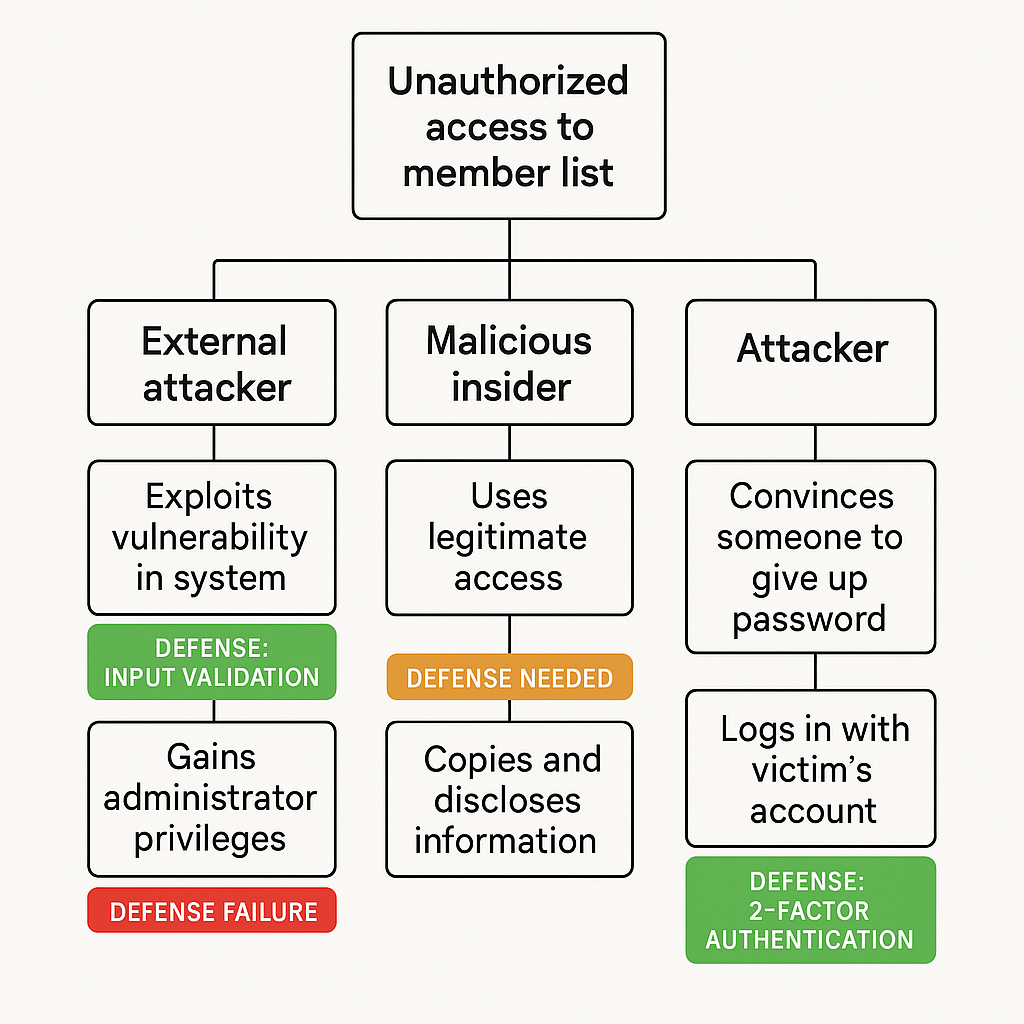
\includegraphics[width=0.6\linewidth]{tree}
        \caption{Attack Tree Example}
        \label{fig:attack_tree_example}
    \end{figure}

    \item \textbf{Conduct Simulations}: Organize simulation exercises for
    more complex scenarios. Assign someone to represent the adversary, while others
    act as defenders or observers. For example, simulate a Sybil attack scenario:
    "Maria secretly created false identities before a vote and uses them to
    influence the results." Go through the steps, discussing whether current
    procedures would detect the attack. This exercise helps reveal weaknesses in a
    safe, low-pressure environment rather than during an actual incident.
    This kind of storytelling helps highlight if your current processes have detection or not.

    \item \textbf{Identify Vulnerabilities at Each Step}: For each scenario,
    explicitly identify the weaknesses that make the attack possible. Include both
    technical issues ("outdated software", "no data backups") and organizational
    issues ("no membership verification", "one person controls critical knowledge").
    Identify your current controls and assess whether they actually prevent the
    attack or whether they can be circumvented. Clearly document these
    vulnerabilities for each scenario, which helps directly inform your mitigation
    efforts.

    \item \textbf{Assess the Impact and Likelihood of Scenarios}: Clearly discuss
    the severity of each scenario and the likelihood of its occurrence. Use simple
    terms: High, Medium, or Low. For example, ransomware that encrypts
    important files may have High Impact due to potential data loss, but only
    Medium Likelihood if members follow best practices. Similarly, a Sybil attack
    may have High Impact due to loss of trust, but Low to Medium Likelihood,
    depending on how carefully you select new members.

    \item \textbf{Leverage Past Incidents}: Incorporate experiences from previous
    incidents or near misses to make scenarios more concrete. Ask, "Could this
    happen again, perhaps in a more damaging way?" For example, "We temporarily lost
    control of our Twitter account before, what if the attackers post harmful content
    next time?" Using real-world examples helps everyone understand the severity of
    the threats and the importance of preventive measures.

\end{itemize}

\subsection{Step 6: Prioritize Risks Together}
\label{subsec:Step6}

Which Problems Matter Most?

\subsubsection{Purpose}

Not all threats are equal. In this step, the group evaluates all the
identified threat scenarios and decides which ones to address first. This is
essentially a risk analysis and ranking. Risk is usually judged by two factors:
how severe the impact would be and how likely the threat is to occur. By scoring
or discussing these, the group can focus on the most critical issues.
Importantly, this is done participatorily, everyone's perspective on what is
important is considered, keeping the process democratic. The output will be a
clear list of top risks that the organization will invest effort in mitigating.

\subsubsection{Activities}

\begin{itemize}

    \item \textbf{Define Impact and Likelihood}: First, agree on clear
    definitions for impact and likelihood. High impact risks threaten the
    organization's survival, break laws, or deeply harm member trust; medium impacts
    create noticeable but manageable problems; low impacts result in minor
    inconveniences. High likelihood means there's strong evidence a risk can easily
    happen, medium is conditional, and low likelihood means it's rare or requires
    sophisticated effort. Use simple terms (high, medium, low), but ensure everyone
    understands them clearly.
    
    \item \textbf{Evaluate Each Threat Scenario}: Review your scenarios from Step 3 to 5 one by one,
    asking two questions: "If this happens, how bad is it? (Impact)" and "How likely
    is it? (Likelihood)." Different perspectives matter,for example, tech members
    might know a threat is difficult to execute (low likelihood), while governance
    experts could emphasize the severe impact on trust. Aim for informal consensus
    or use a voting method to agree on each scenario's risk level.
    
    \item \textbf{Rank the Risks}: Identify the most critical risks needing immediate
    action, usually those with high impact, high likelihood, or both. Pay attention
    also to "easy fixes", issues that might be medium risk but simple to address
    immediately. Classify risks into categories like Critical (fix urgently),
    Moderate (plan action), and Low (acknowledge without immediate action).
    
    \item \textbf{Document Your Reasoning}: Clearly note why each top risk was
    prioritized. For example: "Sybil attack on voting, High Impact (could damage
    governance legitimacy), Low Likelihood (approval required for new members), still
    prioritized due to potential impact on trust". This transparency helps others
    understand the choices later.
    
    \item \textbf{Check Against Goals}: Revisit \hyperref[subsec:Step1]{Step 1's} initial assets and objectives.
    Ensure the prioritized risks align with your core mission and values. If
    important assets lack high-ranked threats, double-check if something was
    overlooked or truly low risk. Likewise, ensure you're not overly prioritizing
    threats unrelated to your central goals.
    
    \item \textbf{Get Group Approval}: Finally, confirm group agreement on your chosen
    top threats. For smaller groups, informal agreement may suffice; larger groups
    might prefer a quick formal vote. This step reinforces collective responsibility
    and accountability for the chosen priorities.

\end{itemize}
    
\subsection{Step 7: Mitigations and Governance Decisions}
\label{subsec:Step7}

How Do We Fix or Prevent Issues?

\subsubsection{Purpose}

For each of the top priority threats, decide on countermeasures and integrate
those decisions into the organization's action plan. In other words, figure out what
security measures to implement and how to approve and enforce them
democratically. This step is where you turn analysis into concrete changes:
technical fixes, new or improved policies, training, etc. It's also where you
make sure that implementing these fixes doesn't accidentally centralize power or
violate cooperative principles.

\subsubsection{Activities}

\begin{itemize}

    \item \textbf{Brainstorm Mitigation Options:} For each high priority threat,
    list potential mitigations. These might include technical solutions (software
    updates, two-factor authentication, encryption), workflow improvements
    (clear onboarding/offboarding processes, regular backups, peer reviews
    for critical tasks), training and education (phishing awareness, password
    management sessions, annual security policy orientations), and governance
    policies (formal rules for password storage, emergency decision protocols,
    member identity verification).
    
    \item \textbf{Evaluate Feasibility:} Consider the practicality of each
    mitigation. Discuss how difficult or costly they are, if external resources are
    required, if they introduce significant workflow friction, and if they align
    with organizational values. Use adversary personas to check effectiveness, ask if
    specific measures effectively deter identified threats.
    
    \item \textbf{Deliberate and Decide Collectively:} Engage members or relevant
    subgroups to choose appropriate mitigations. Include those responsible for
    implementation and those affected by changes. Address concerns through
    discussion, propose alternative solutions, and aim for consensus. Document
    clearly why each chosen mitigation was prioritized.
    
    \item \textbf{Assign Responsibilities Clearly:} Define clear responsibilities
    for each mitigation task, distributing them among relevant members or working
    groups. Technical tasks should include tech-skilled members paired with others
    for transparency. Assign policy drafting and educational roles to suitable teams
    or individuals. Clearly state budget needs for specific tasks to ensure
    alignment with cooperative budgeting processes.
    
    \item \textbf{Implement with Democratic Oversight:} Keep the organization
    updated throughout the implementation process. Regularly report progress in
    meetings or group communications. Drafted policies should circulate for
    collective review and formal adoption. Ensure full cooperation from members,
    emphasizing that security measures result from collective decisions.
    
    \item \textbf{Prepare for Emergencies:} Establish clear protocols for crisis
    situations requiring rapid response. Formally designate a small emergency
    response team authorized to take quick decisions within agreed limits. Define
    the scope and timeframe for their actions, and ensure accountability by
    mandating transparent post-incident reporting and collective decision making on
    permanent actions.
    
    \item \textbf{Integrate into Governance Documents:} Codify agreed-upon
    mitigations and emergency protocols into the organization's official
    documentation. Update handbooks or wikis to institutionalize these practices,
    ensuring new members receive proper orientation.
    
    \item \textbf{Set Review Milestones:} Schedule periodic reviews to assess the
    effectiveness and implementation status of security measures. Quick check-ins at
    regular meetings, formal reviews after a set period, or integration into annual
    reviews help maintain accountability and adapt strategies as needed.
    
\end{itemize}

\subsection{Participation Tips}
\label{subsec:participation_tips}

Successful threat modeling requires that everyone in the organization feels comfortable
and motivated to contribute. In small groups, completing activities in a single meeting is
effective, fostering unity and avoiding repeat sessions. For larger groups, use
brief questionnaires or small group discussions, consolidating ideas later in
plenary to ensure that everyone can contribute.

It is important that members with technical expertise do not dominate the
conversation. Encourage more reserved participants by asking them directly for
their opinions on specific threats or solutions.

Keep a relaxed and creative environment when role-playing scenarios or
developing adversarial personas and document decisions transparently,
explaining the reasons clearly, allowing for future review and improvements.

Once security measures are in place, encourage open feedback on any challenges
or improvements needed. Share responsibilities equally among team members to
avoid overload, foster collective ownership, and maintain a genuinely flat
organizational structure.

\section*{}
Chapter 4 presented the protocol specifically aimed at
threat modeling in horizontal organizations, detailing fundamental security and
governance requirements. The importance of aligning technological and
organizational processes to ensure robustness against internal and
external threats was highlighted. Based on this conceptual
development, Chapter 5 summarizes the main results achieved by this research,
critically evaluating the proposed protocol, identifying its contributions in
relation to traditional methodologies, and exploring practical applications in real environments.
